% !TeX spellcheck = en_US
\chapter{\iceact Simulation}\label{chap:iceact_sim}

This chapter will discuss the \geant simulation process. \todo{bisschen mehr?}

\section{Simulation of Single Components}

In order to make some first checks and optimization, the focus is on single essential components, i.e. the Fresnel lens and the Winston cones.

\subsection{\enquote{Best} Wavelength}\label{sec:best_wvl}

Many of the \iceact telescope properties have (non-linear) wavelength dependencies (cf. section~\ref{sec:iceact:model:material}). Additionally, the Cherenkov spectrum is wavelength dependent as well (cf. figure~\ref{airshowers:cherenkovspectrum}). By implication, there has to be a wavelength $\lambda^\ast$ that \iceact is the most efficient. One can determine $\lambda^\ast$ by looking at the following limiting functions.

\begin{itemize}
	\item The Cherenkov spectrum. The data shown in figure~\ref{airshowers:cherenkovspectrum} (La Palma, \SI{2200}{\meter} a.s.l.) is chosen.
	\item The internal transmission function of PMMA. It is assumed that a photon has to pass approximately \SI{30}{\milli\meter} of PMMA to get to the SiPMs. Thus, the internal transmission function shown in figure~\ref{iceact:model:material:transmission} as blue dotted-dashed line has to be exponentiated by \num{10} to hold for this case.
	\item The internal transmission function of borosilicate, i.e. the material of the glass plate. The photons have to pass approximately \SI{2}{\milli\meter}. Exponentiation of a factor $\frac{2}{3}$ of the orange dotted-dashed line in figure~\ref{iceact:model:material:transmission} leads to the desired function.
	\item The photon detection efficiency (PDE) function of the SiPMs interpolated for $V_\text{OV} = \SI{5}{\volt}$ (cf. orange curve in figure~\ref{sipm:pde}).
\end{itemize}

All of these functions are normalized, i.e. divided by their own maximum, and than multiplied which results in a new (relative) efficiency function. The maximum of this function again is the \enquote{best} wavelength found to be $\lambda^\ast = \SI{411}{\nano\meter}$. Figure~\ref{best_wvl} shows the procedure graphically. 

\begin{figure}[H]
	\centering
	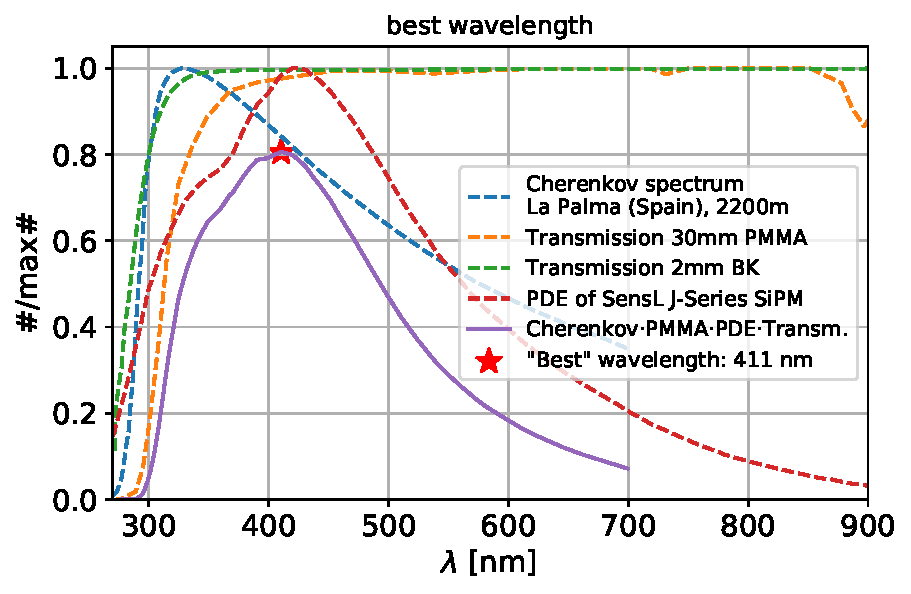
\includegraphics[width=0.7\textwidth]{best_wvl.pdf}
	\caption[\enquote{Best} wavelength]{\textbf{\enquote{Best} wavelength.} All limiting functions (Cherenkov spectrum, matrial transmission curves, and photon detection efficiency) are nomalized to each maximum and multiplied. The maximum of the product is defined to be the \enquote{best}, i.e. most efficient, wavelength $\lambda^\ast=\SI{411}{\nano\meter}$.}
	\label{best_wvl}
\end{figure}

\subsection{Focal Plane Shift}\label{sec:focalplaneshift}

So there is a most efficient wavelength for the \iceact telescope as shown in the last section~\ref{sec:best_wvl}. As stated in section~\ref{iceact:model:fresnellens} and in the ORAFOL data sheet~\cite{iceact:fresnellens:datasheet}, the focal distance of the Fresnel lens $z_f=\SI{502.1}{\milli\meter}$ is given for a certain wavelength $\lambda=\SI{546+-27.3}{\nano\meter}$. Thus, the focal distance at $\lambda^\ast=\SI{411}{\nano\meter}$ may be different which gives a possibility for potential improvement for the optical properties of \iceact. To investigate a shift of the focal plane, one has to define a quantity to optimize. In this simulation, the aberration radius $r_{90}$ is used for this purpose (cf. section~\ref{iceact:model:fresnellens}). A point spread function measurement of the Fresnel lens for monochromatic light with $\lambda=\SI{546}{\nano\meter}$ and different incidence angles $\theta$ is done in~\cite{famous:niggemann} by using ray tracing simulation. In this thesis, a PSF simulation is done as well but for wavelengths between $\SI{270}{\nano\meter}$ and $\SI{900}{\nano\meter}$ and vertical incidence $\theta=\SI{0}{\degree}$. The focal plane is fixed at the focal distance $z_f=\SI{502.1}{\milli\meter}$. In total, a vertical beam of \num{1e8} photons with uniformly density and uniformly distributed wavelengths in the interval given above is simulated. On the focal plane, the wavelength $\lambda_\text{hit}$, position $(x_\text{hit},y_\text{hit}))$, and angle $(\theta_\text{hit},\phi_\text{hit})$ of the detected photons are registered. The goal is to measure the minimal aberration radius at the suggested focal distance $z_f=\SI{502.1}{\milli\meter}$ and a possible focal plane shift in order to minimize the aberration radius for $\lambda^\ast=\SI{411}{\nano\meter}$.\\

For the first measurement, the aberration radius is evaluated by calculating the \SI{90}{\percent}-quantile of the distances $r_\text{hit}$ between the hit position and the optical axis\footnote{Normally, this is the centroid rather than the optical axis but in the case of parallel light, the centroid is assumed to be at $(x,y) = (0,0)$.} given by
\begin{align}
	r_\text{hit} = \sqrt{\left(x_\text{hit}-x_\text{centroid}\right)^2+\left(y_\text{hit}-y_\text{centroid}\right)^2} \overset{(x,y)_\text{centroid}=(0,0)}{=}\sqrt{x_\text{hit}^2+y_\text{hit}^2}\,.
\end{align}
By doing this for small wavelength ranges, one gets a wavelength-dependent aberration radius $r_{90}(\lambda)$ on the focal plane. As a result, a minimal aberration radius of \SI{1.78}{\milli\meter} is reached at a wavelength of \SI{403}{\nano\meter}. Figure~\ref{psf_at_focal_plane} shows $r_{90}(\lambda)$.\\

\begin{figure}[H]
	\centering
	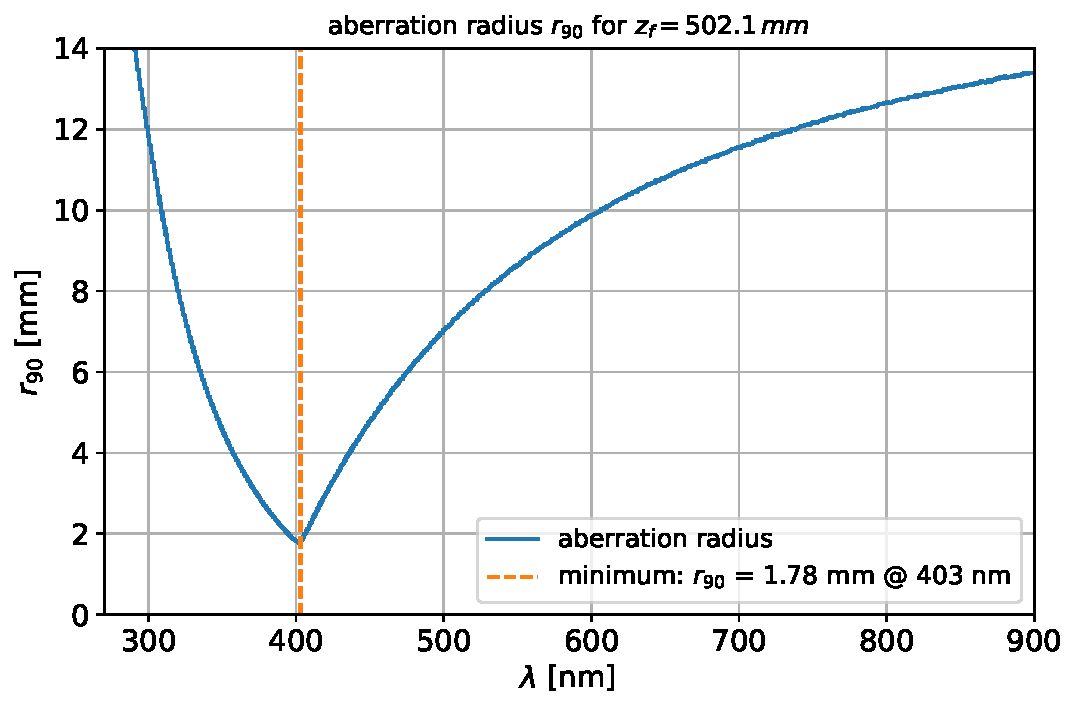
\includegraphics[width=0.8\textwidth]{focalplaneshift/psf_r90.pdf}
	\caption[Aberration radius on the focal plane]{\textbf{Aberration radius on the focal plane.} $r_{90}$ is calculated for vertical light as a function of the wavelength. The focal distance is fixed to $z_f=\SI{502.1}{\milli\meter}$. The minimal aberration radius of \SI{1.78}{\milli\meter} is reached at a wavelength of \SI{403}{\nano\meter}.}
	\label{psf_at_focal_plane}
\end{figure}

For the focal plane shift, one considers a small wavelength range and again calculates the aberration radius. Since the incidence angles on the focal plane are known, one can calculate the point of incidence for a hypothetical focal plane at a position of $z_f+\Delta z$, where $\Delta z$ is the focal plane shift. A trigonometrical approach gives
\begin{align}
	r_\text{hit}(\Delta z) = \sqrt{\left(x_\text{hit}-\Delta z\tan\theta_\text{hit}\cos\phi_\text{hit}\right)^2 + \left(y_\text{hit}-\Delta z\tan\theta_\text{hit}\sin\phi_\text{hit}\right)^2}\,.
\end{align}
Thus, the aberration radius can be calculated for each focal plane shift $\Delta z$ and wavelength $\lambda$. Than, an optimal focal plane shift can be found by minimizing the aberration radius. Figure~\ref{focalplaneshift} shows this calculation for different wavelengths by evaluation the beam \enquote{caustic}\footnote{In this context, caustic means the photon density distribution along the optical axis. Usually in beam optics, a caustic just describes the envelope of the beam.} for different focal plane shifts. One can clearly see that the focal length increases with wavelength. Additionally, figure~\ref{focalplaneshift_zoomout} shows a zoomed-out version of figure~\ref{focalplaneshift_bestwvl}. In particular for the most efficient wavelength $\lambda^\ast=\SI{411}{\nano\meter}$, a resulting marginal focal plane shift of $\Delta z=\SI{1.25}{\milli\meter}$ shows, that the standard focal distance is already quite good for \iceact. Nevertheless, the focal plane shift is considered in the final parameterization simulation.

\begin{figure}[H]
	\centering
	\begin{subfigure}[t]{0.48\textwidth}
		\centering
		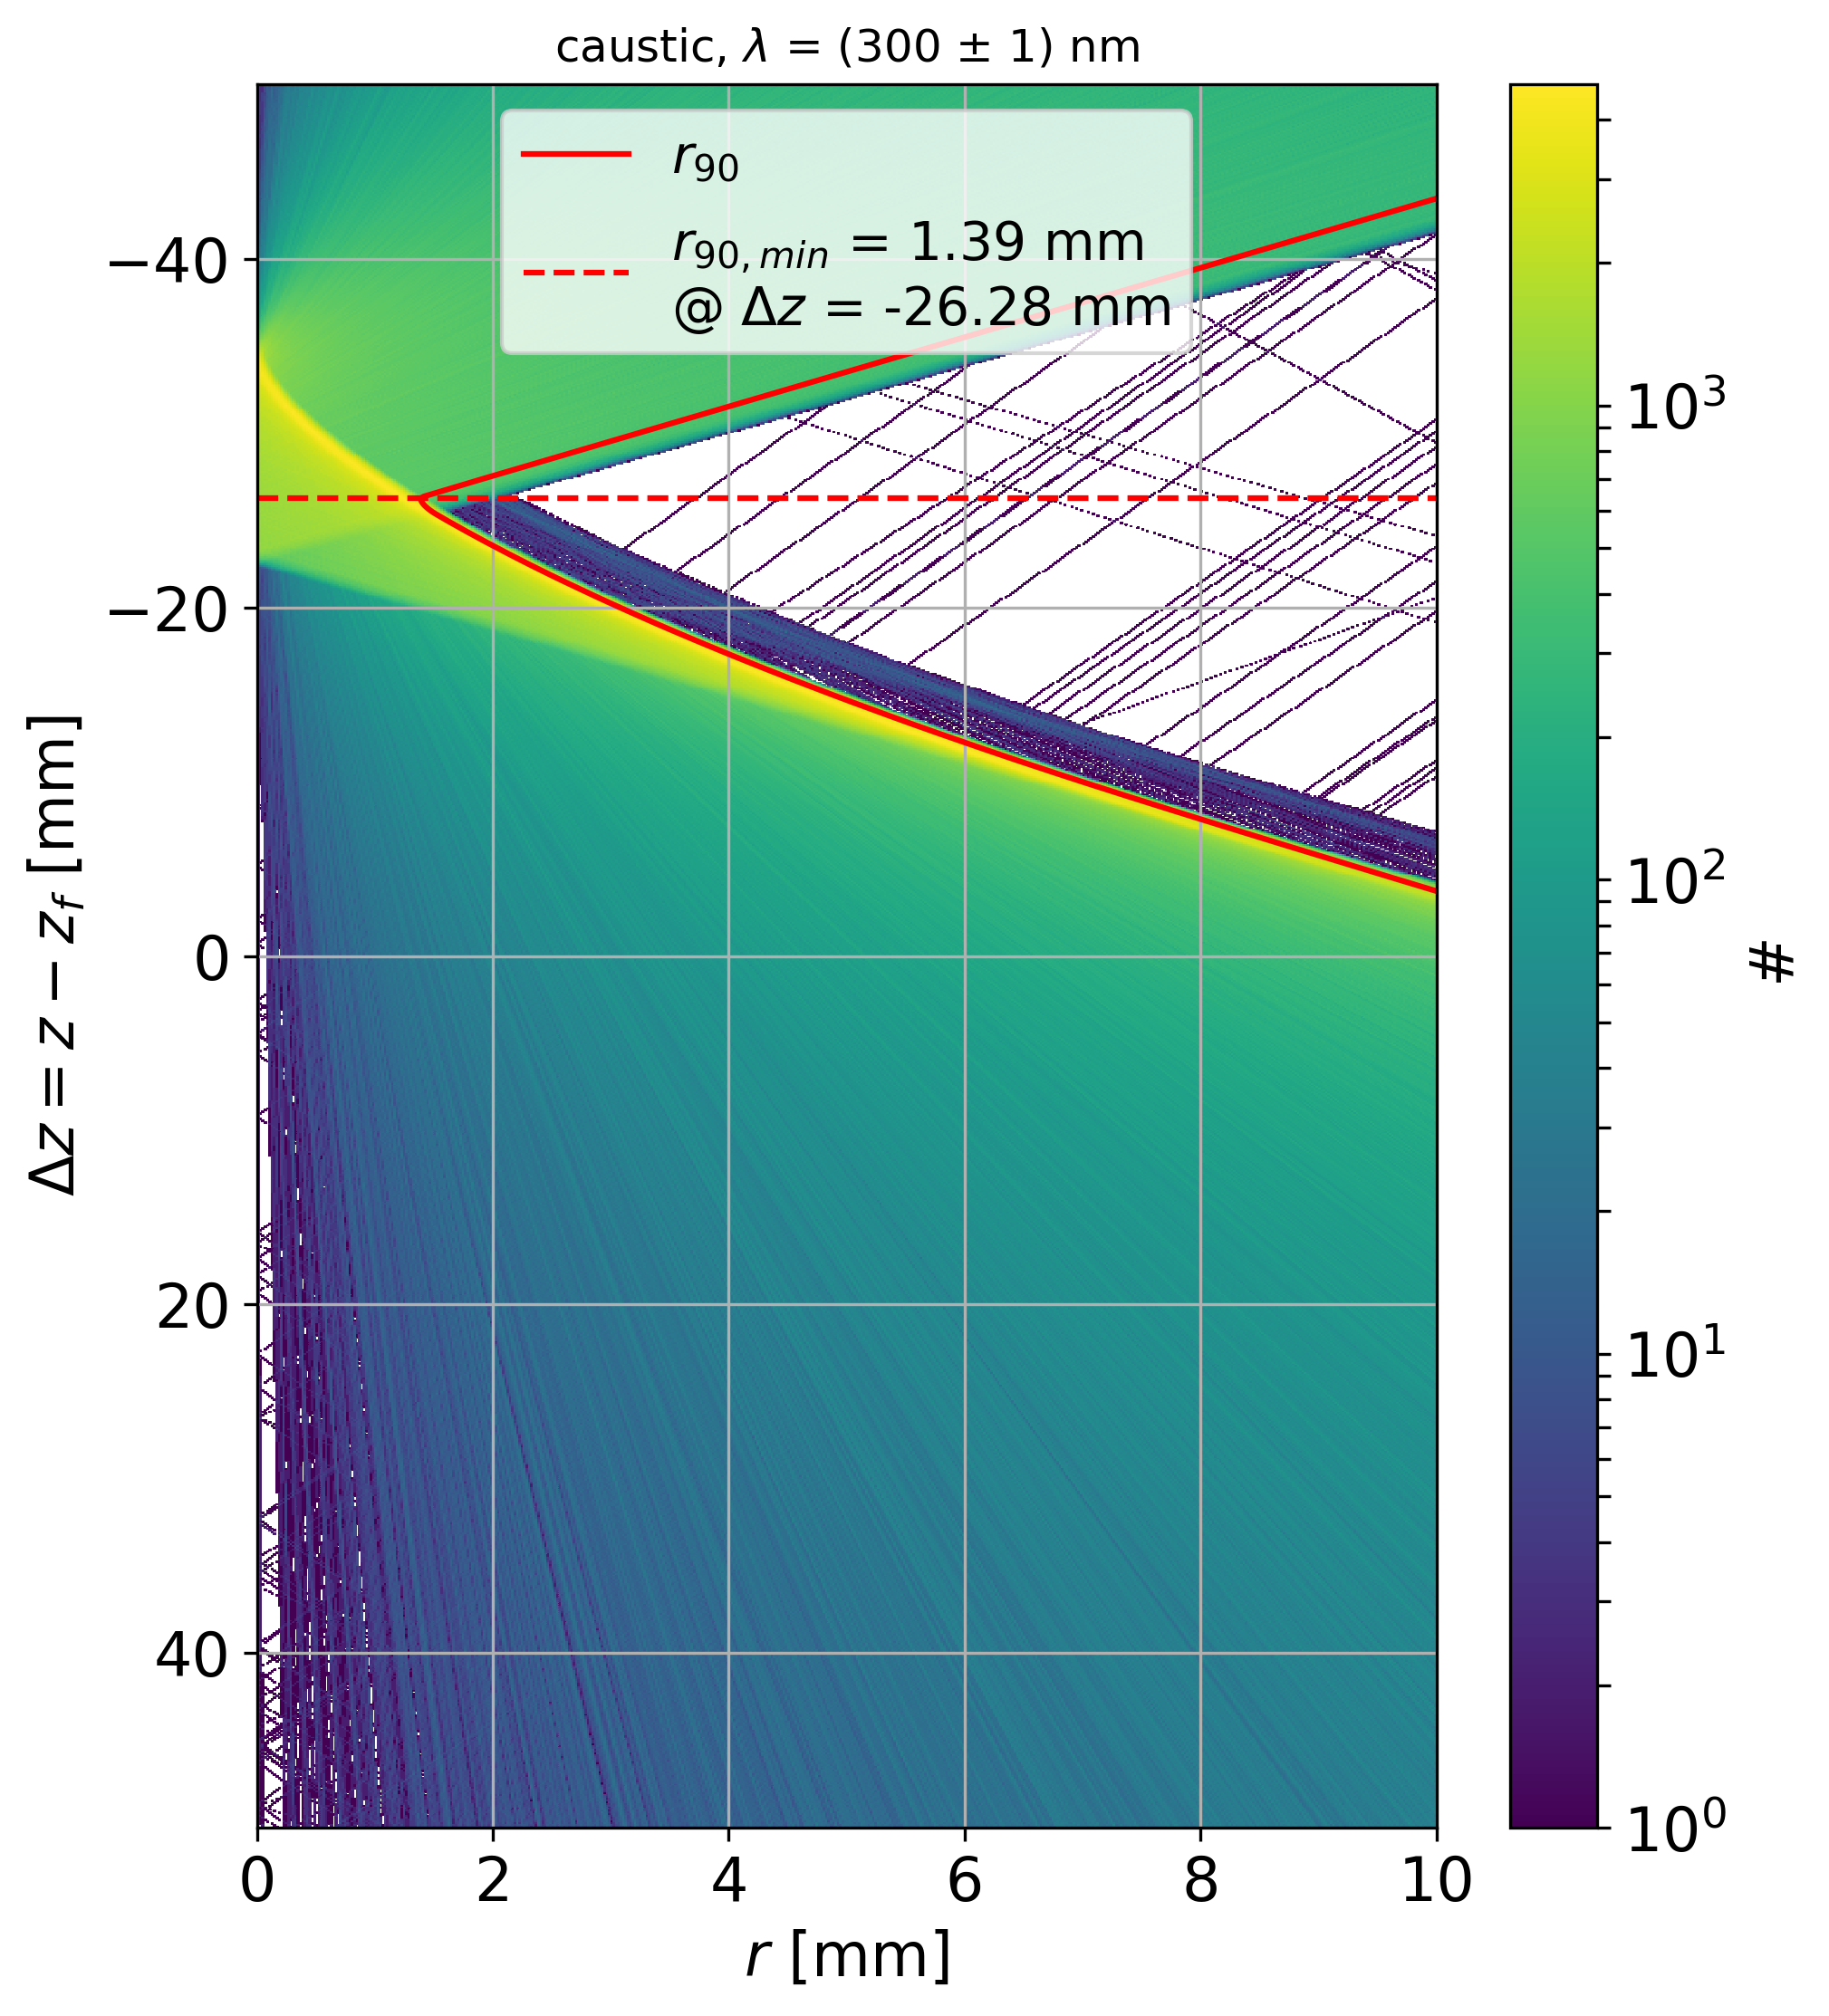
\includegraphics[width=\textwidth]{focalplaneshift/caustic_300nm.png}
		\subcaption{$\lambda=\SI{300+-1}{\nano\meter}$}
	\end{subfigure}
	\hfill
	\begin{subfigure}[t]{0.48\textwidth}
		\centering
		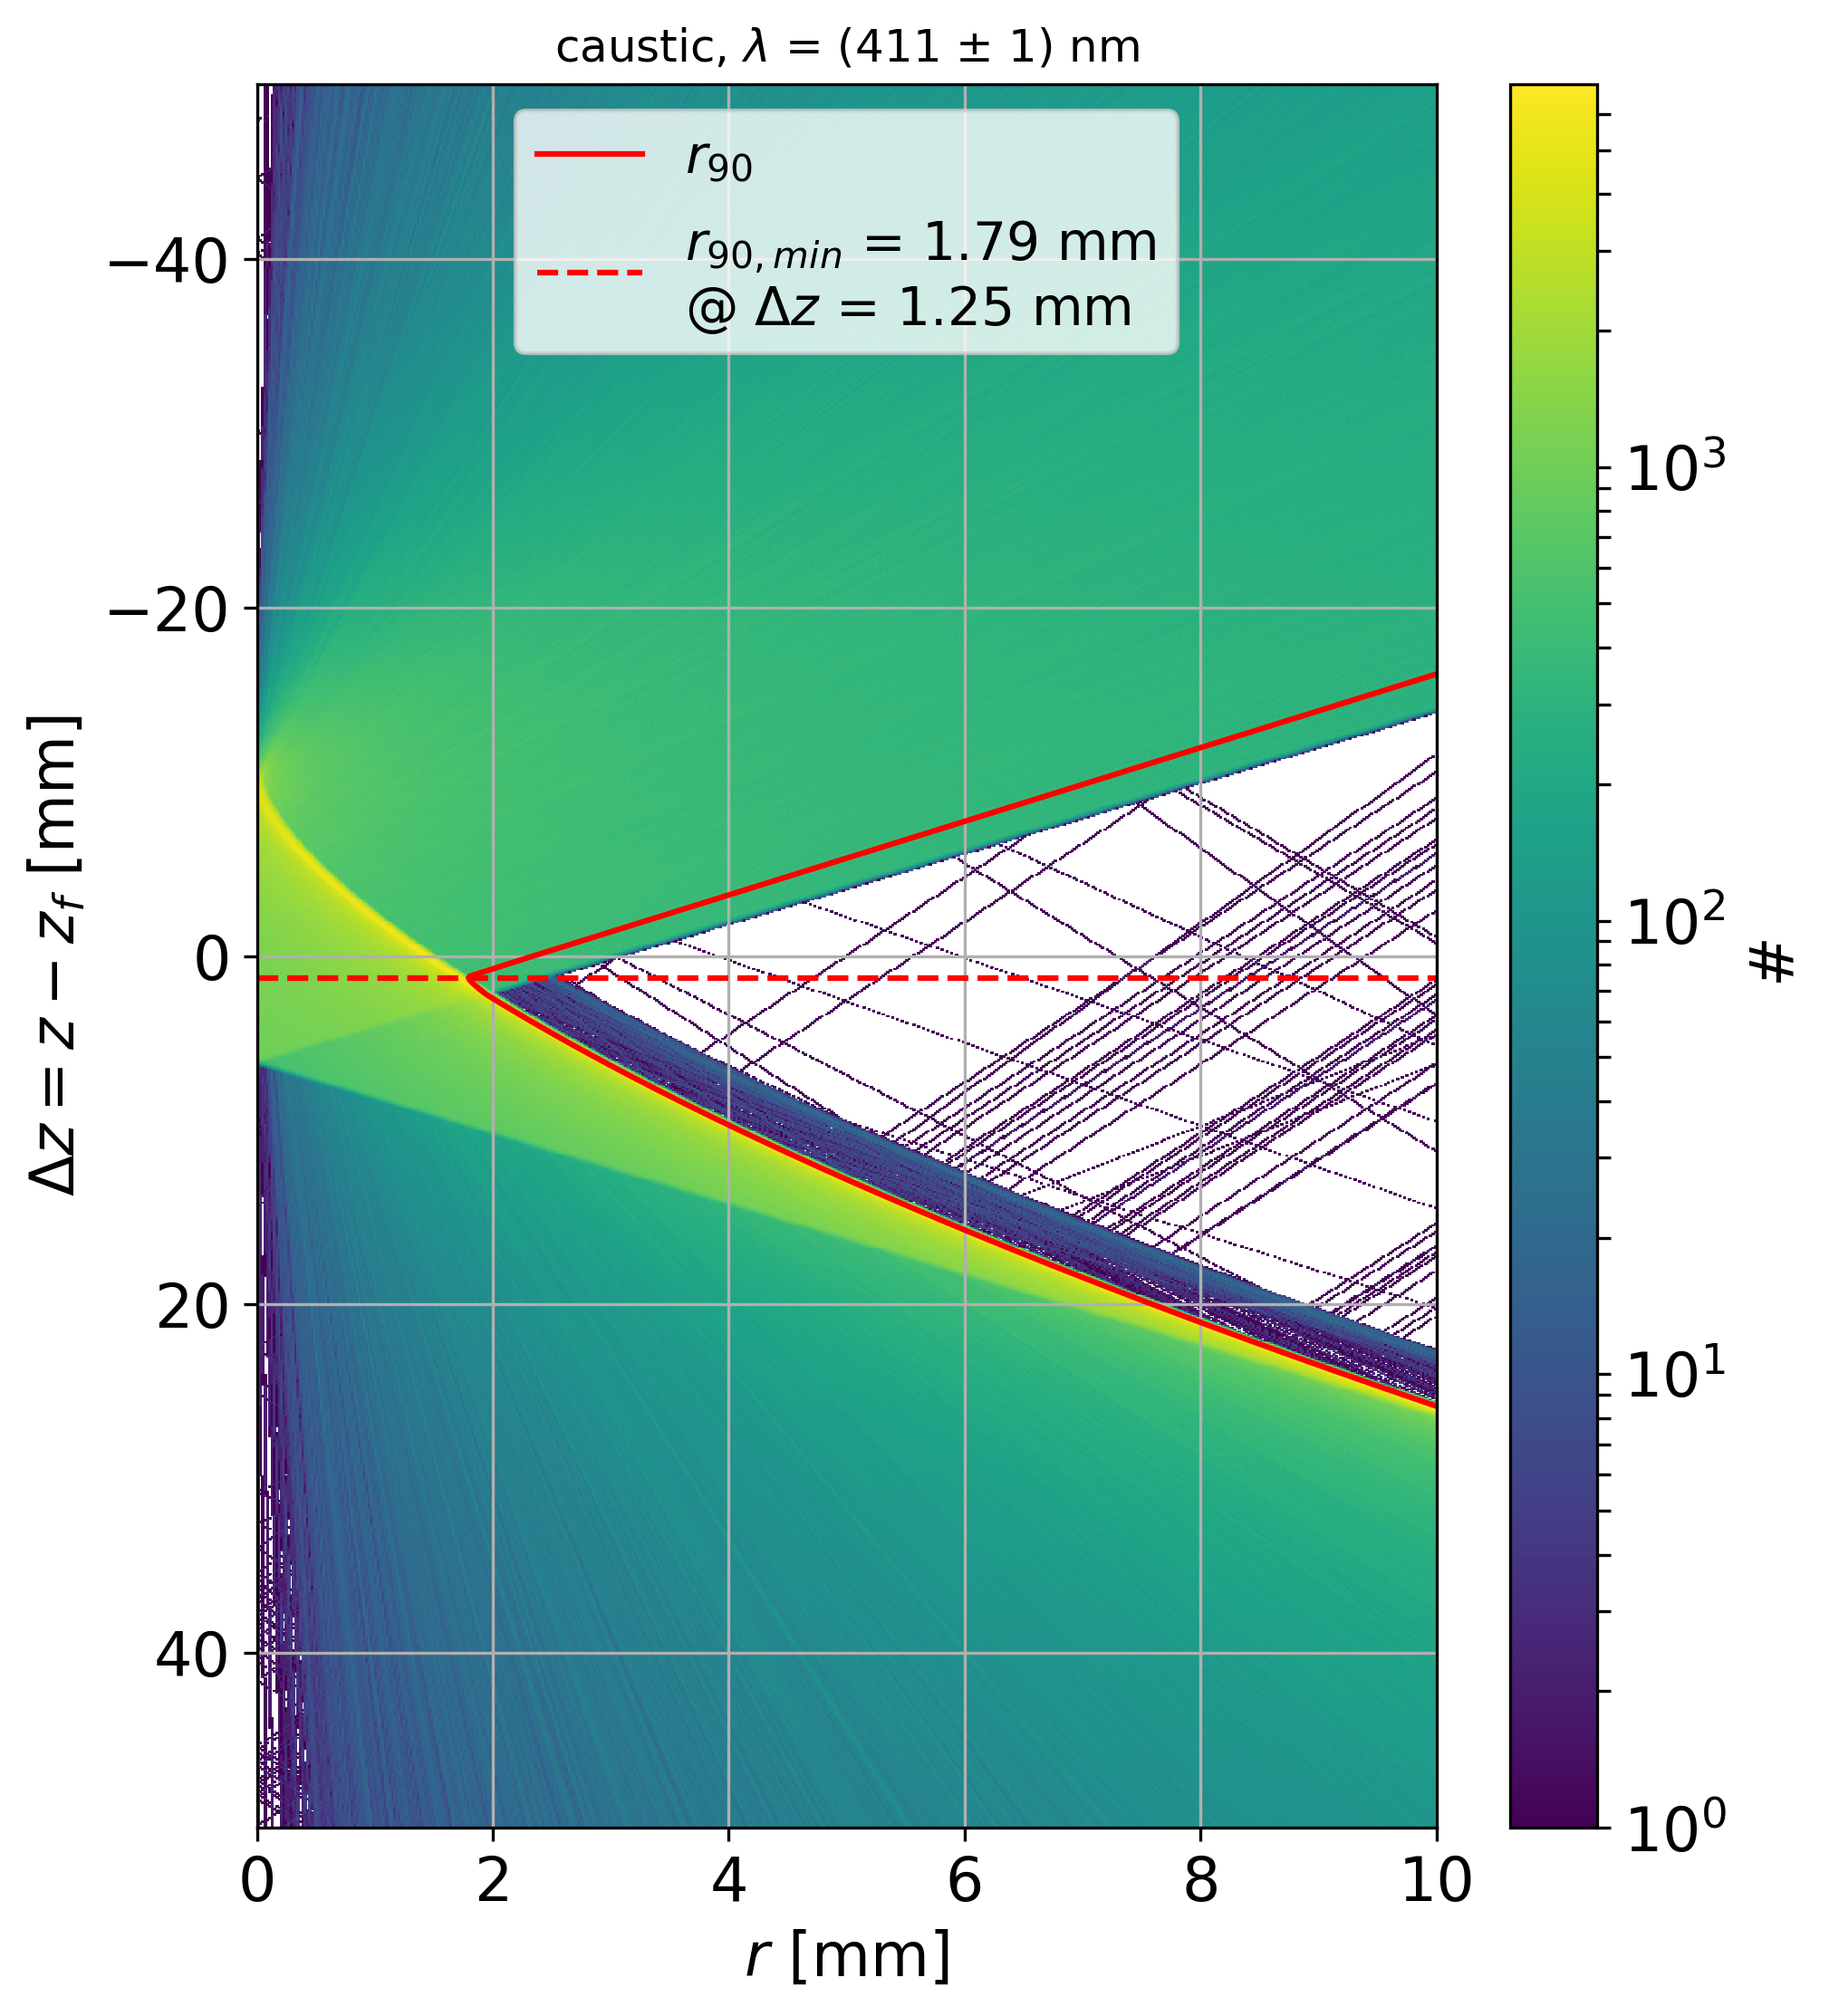
\includegraphics[width=\textwidth]{focalplaneshift/caustic_411nm.png}
		\subcaption{$\lambda^\ast=\SI{411+-1}{\nano\meter}$}
		\label{focalplaneshift_bestwvl}
	\end{subfigure}
	\hfill
	\begin{subfigure}[t]{0.48\textwidth}
		\centering
		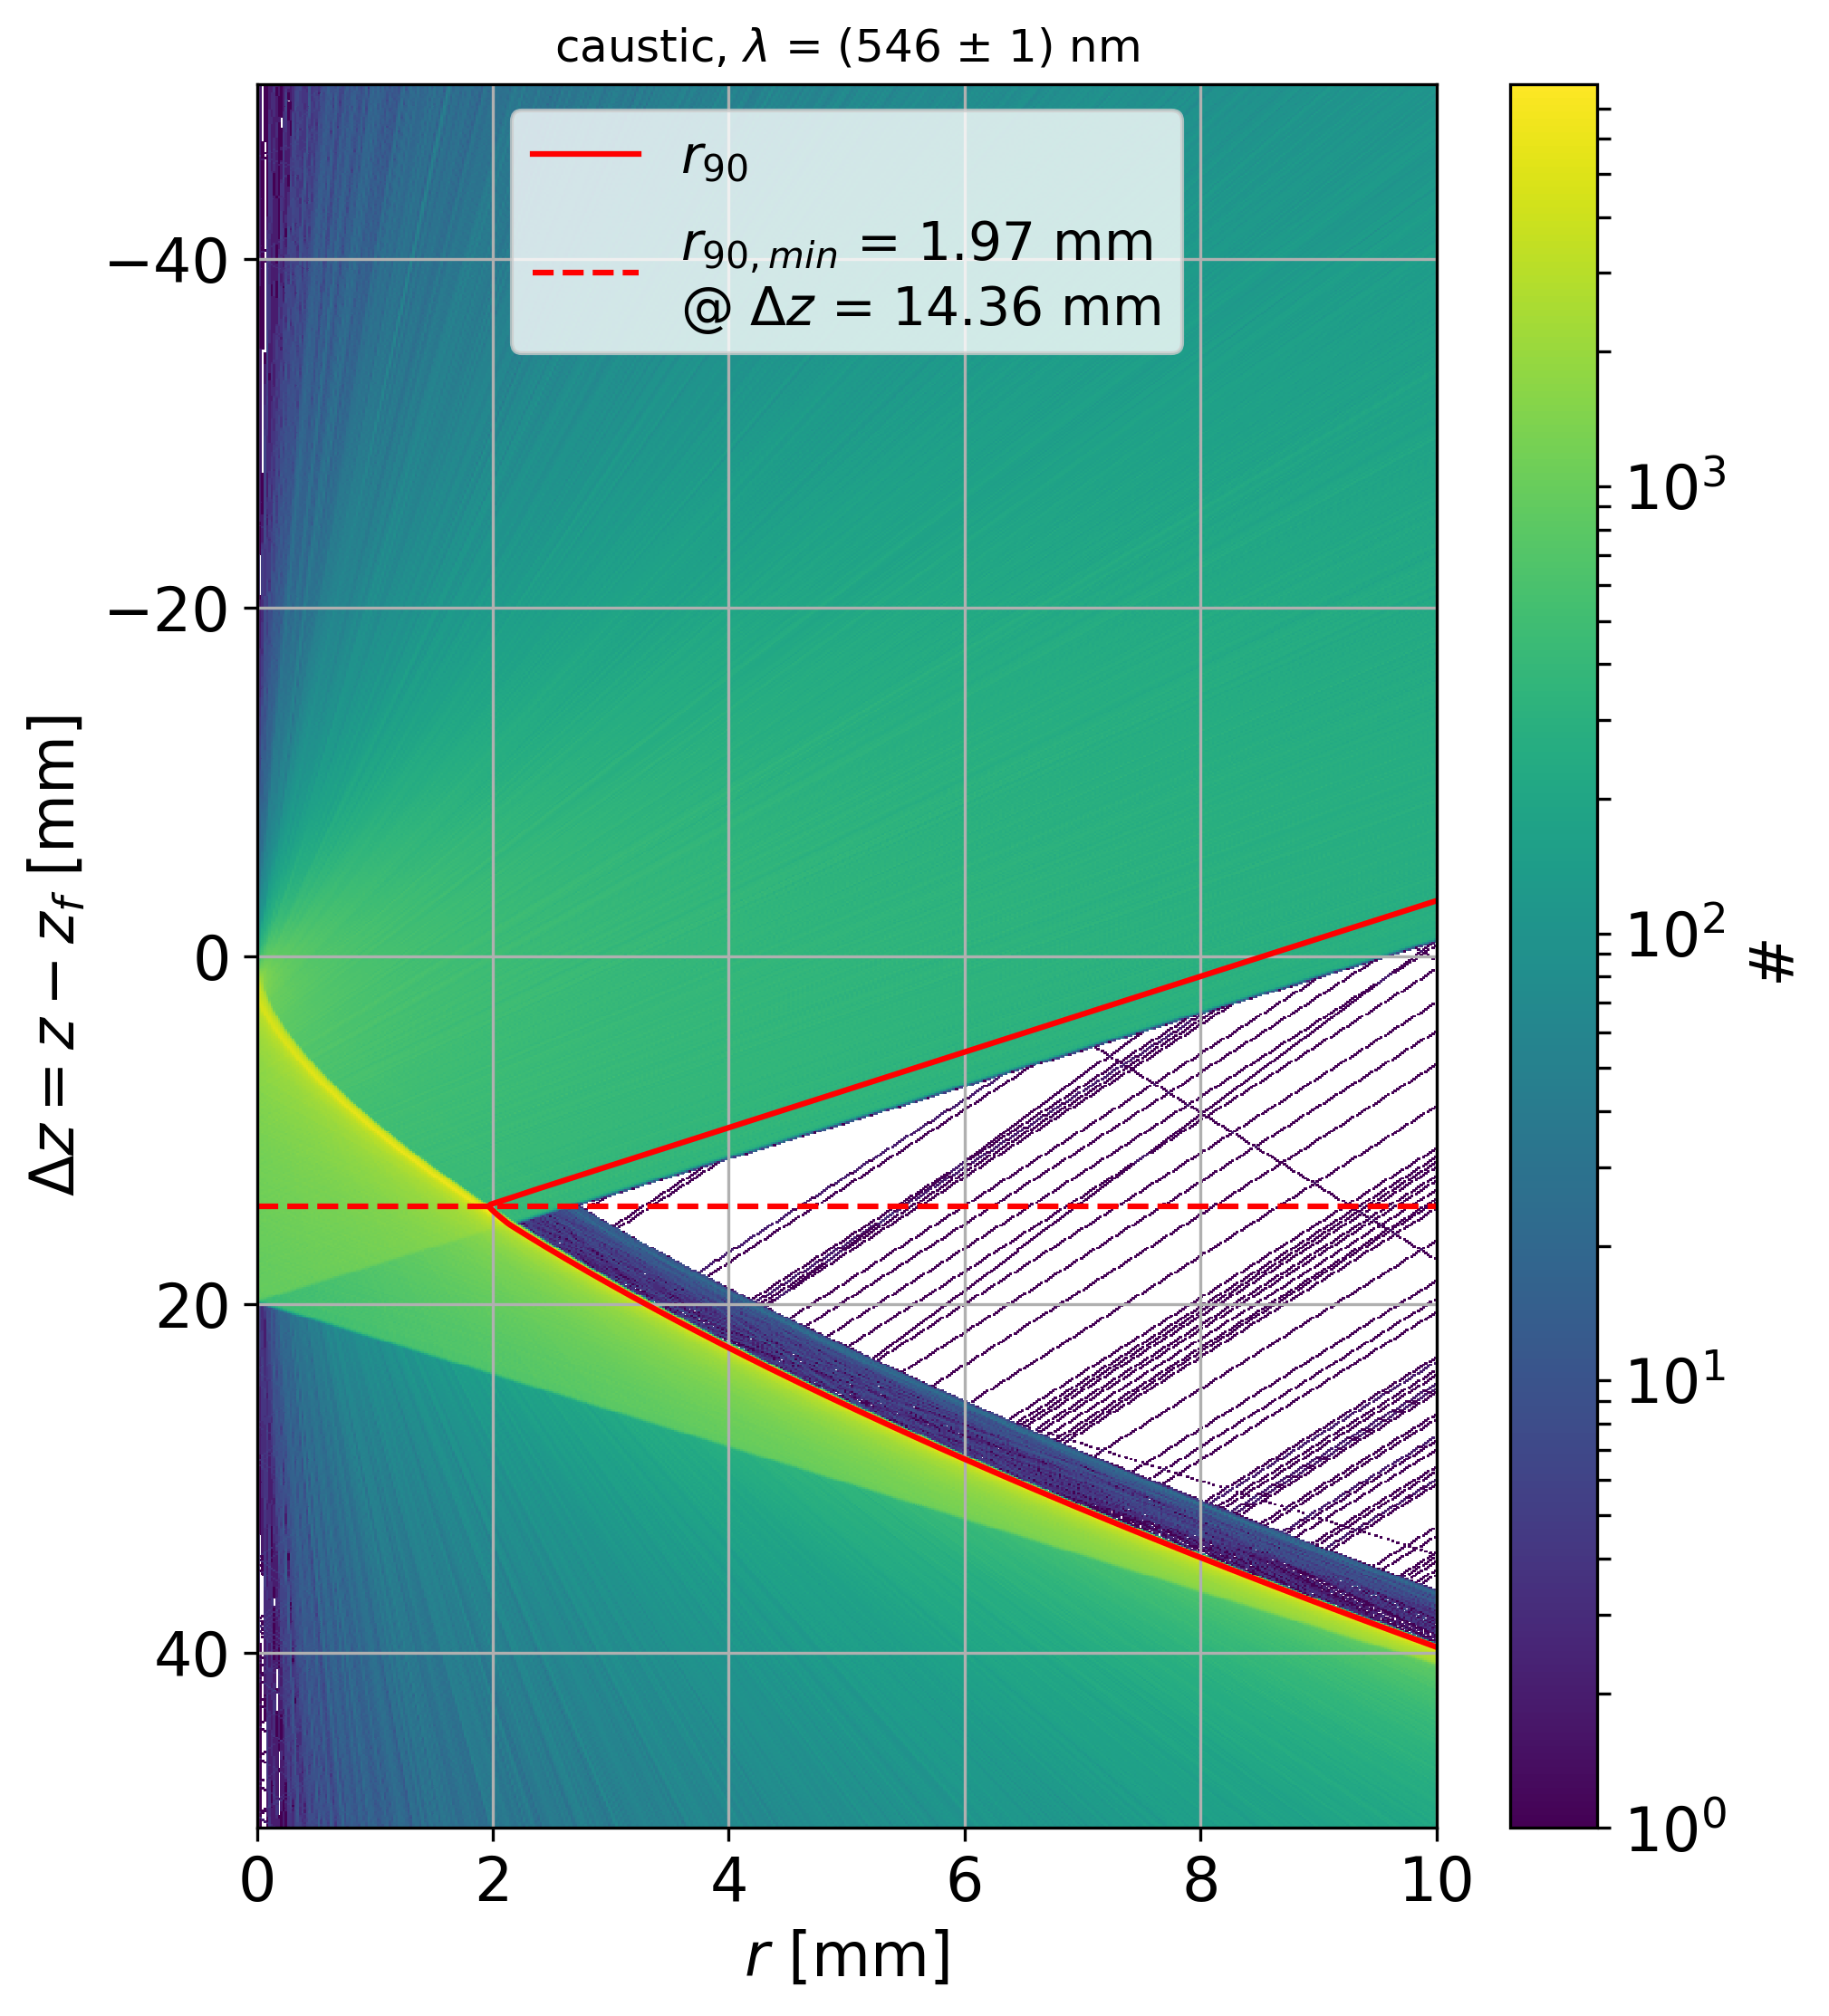
\includegraphics[width=\textwidth]{focalplaneshift/caustic_546nm.png}
		\subcaption{$\lambda=\SI{546+-1}{\nano\meter}$}
		\label{focalplaneshift_famouswvl}
	\end{subfigure}
	\hfill
	\begin{subfigure}[t]{0.48\textwidth}
		\centering
		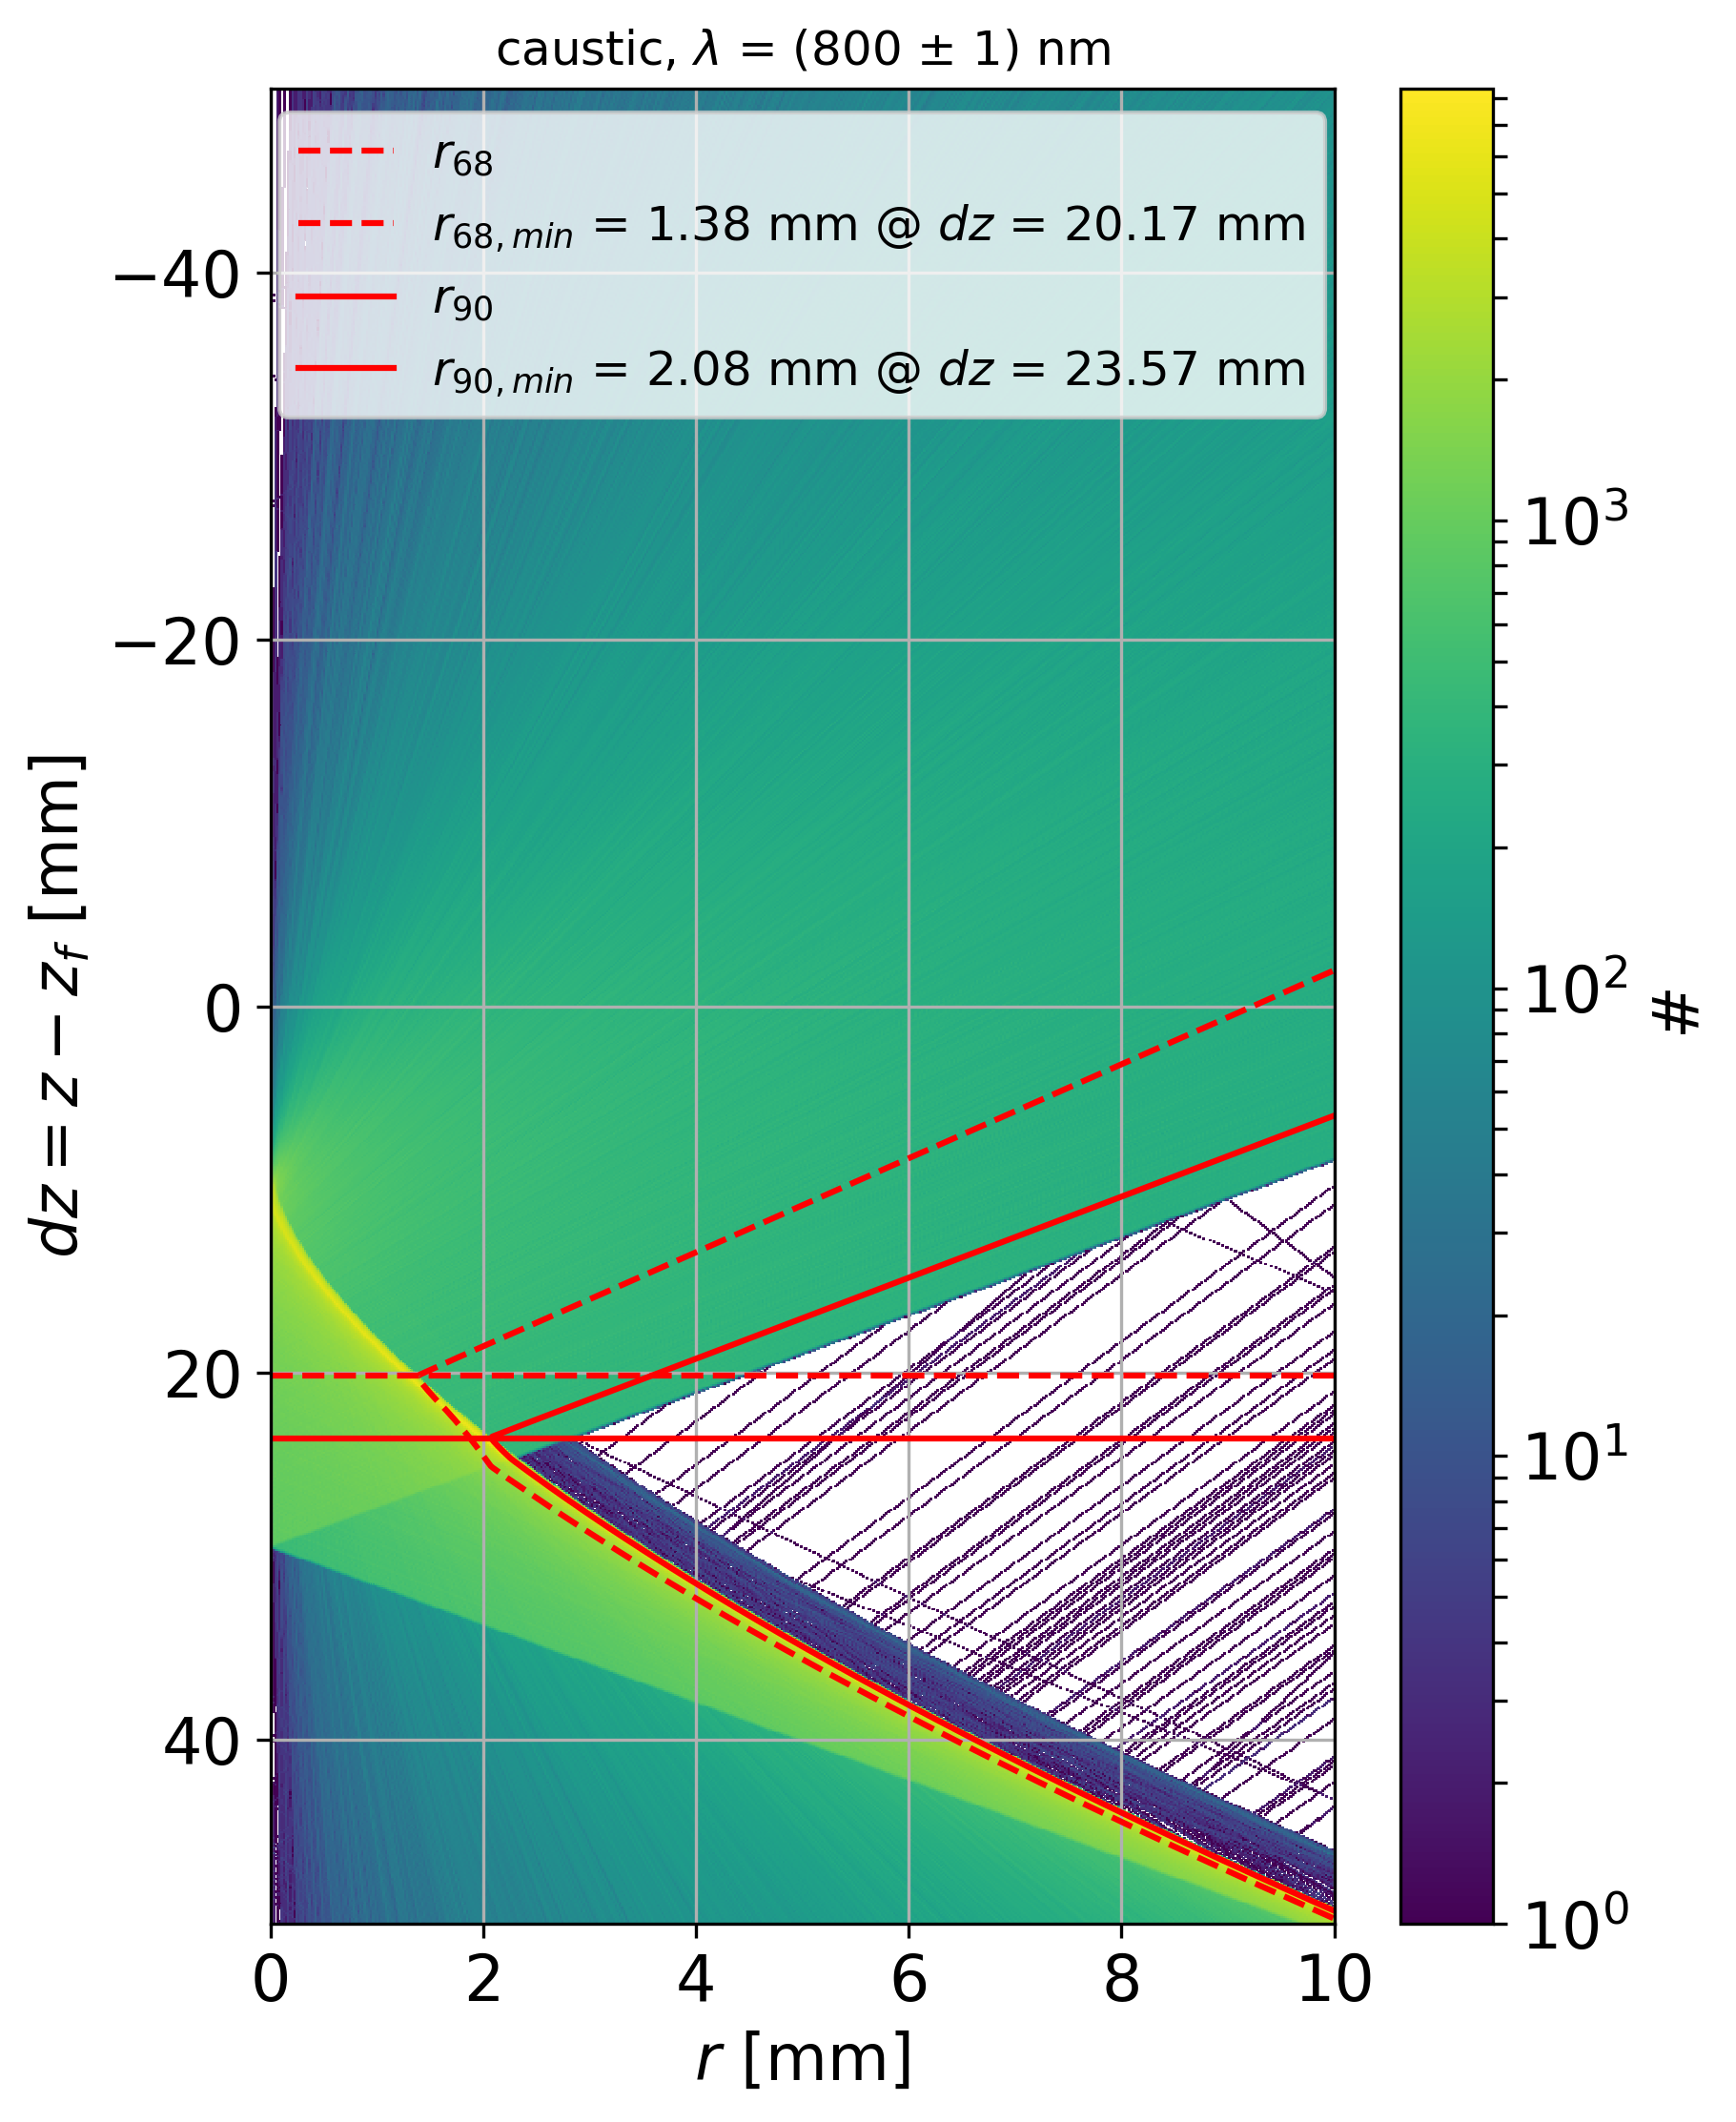
\includegraphics[width=\textwidth]{focalplaneshift/caustic_800nm.png}
		\subcaption{$\lambda=\SI{800+-1}{\nano\meter}$}
	\end{subfigure}
	\caption[\enquote{Caustic} histograms for the focal plane shift]{\textbf{\enquote{Caustic} histograms for the focal plane shift.} For focal plane shifts~$\Delta z$ between $\SI{-50}{\milli\meter}$ and $\SI{50}{\milli\meter}$, the incident positions of simulated photons are histrogramized by calculating their distance from the optical axis $r_\text{hit}(\Delta z)$. This results in a photon density plot called \enquote{caustic}. A focal plane shift of $\Delta z = 0$ is equivalent to the \enquote{standard} focal distance $z_f=\SI{502.1}{\milli\meter}$. A positive $\Delta z$ connotes a shift away from the lens. Thus, the lens is located on top of the shown plots. The calculation is done for different wavelengths, especially for the \enquote{best} wavelength in (\subref{focalplaneshift_bestwvl}) and for the wavelength which the focal distance is set for in (\subref{focalplaneshift_famouswvl}). The red line shows the aberration radius $r_{90}(\Delta z)$ and the focal plane shift where its minimum is reached marked by the red dashed line.}
	\label{focalplaneshift}
\end{figure}

\begin{figure}[H]
	\centering
	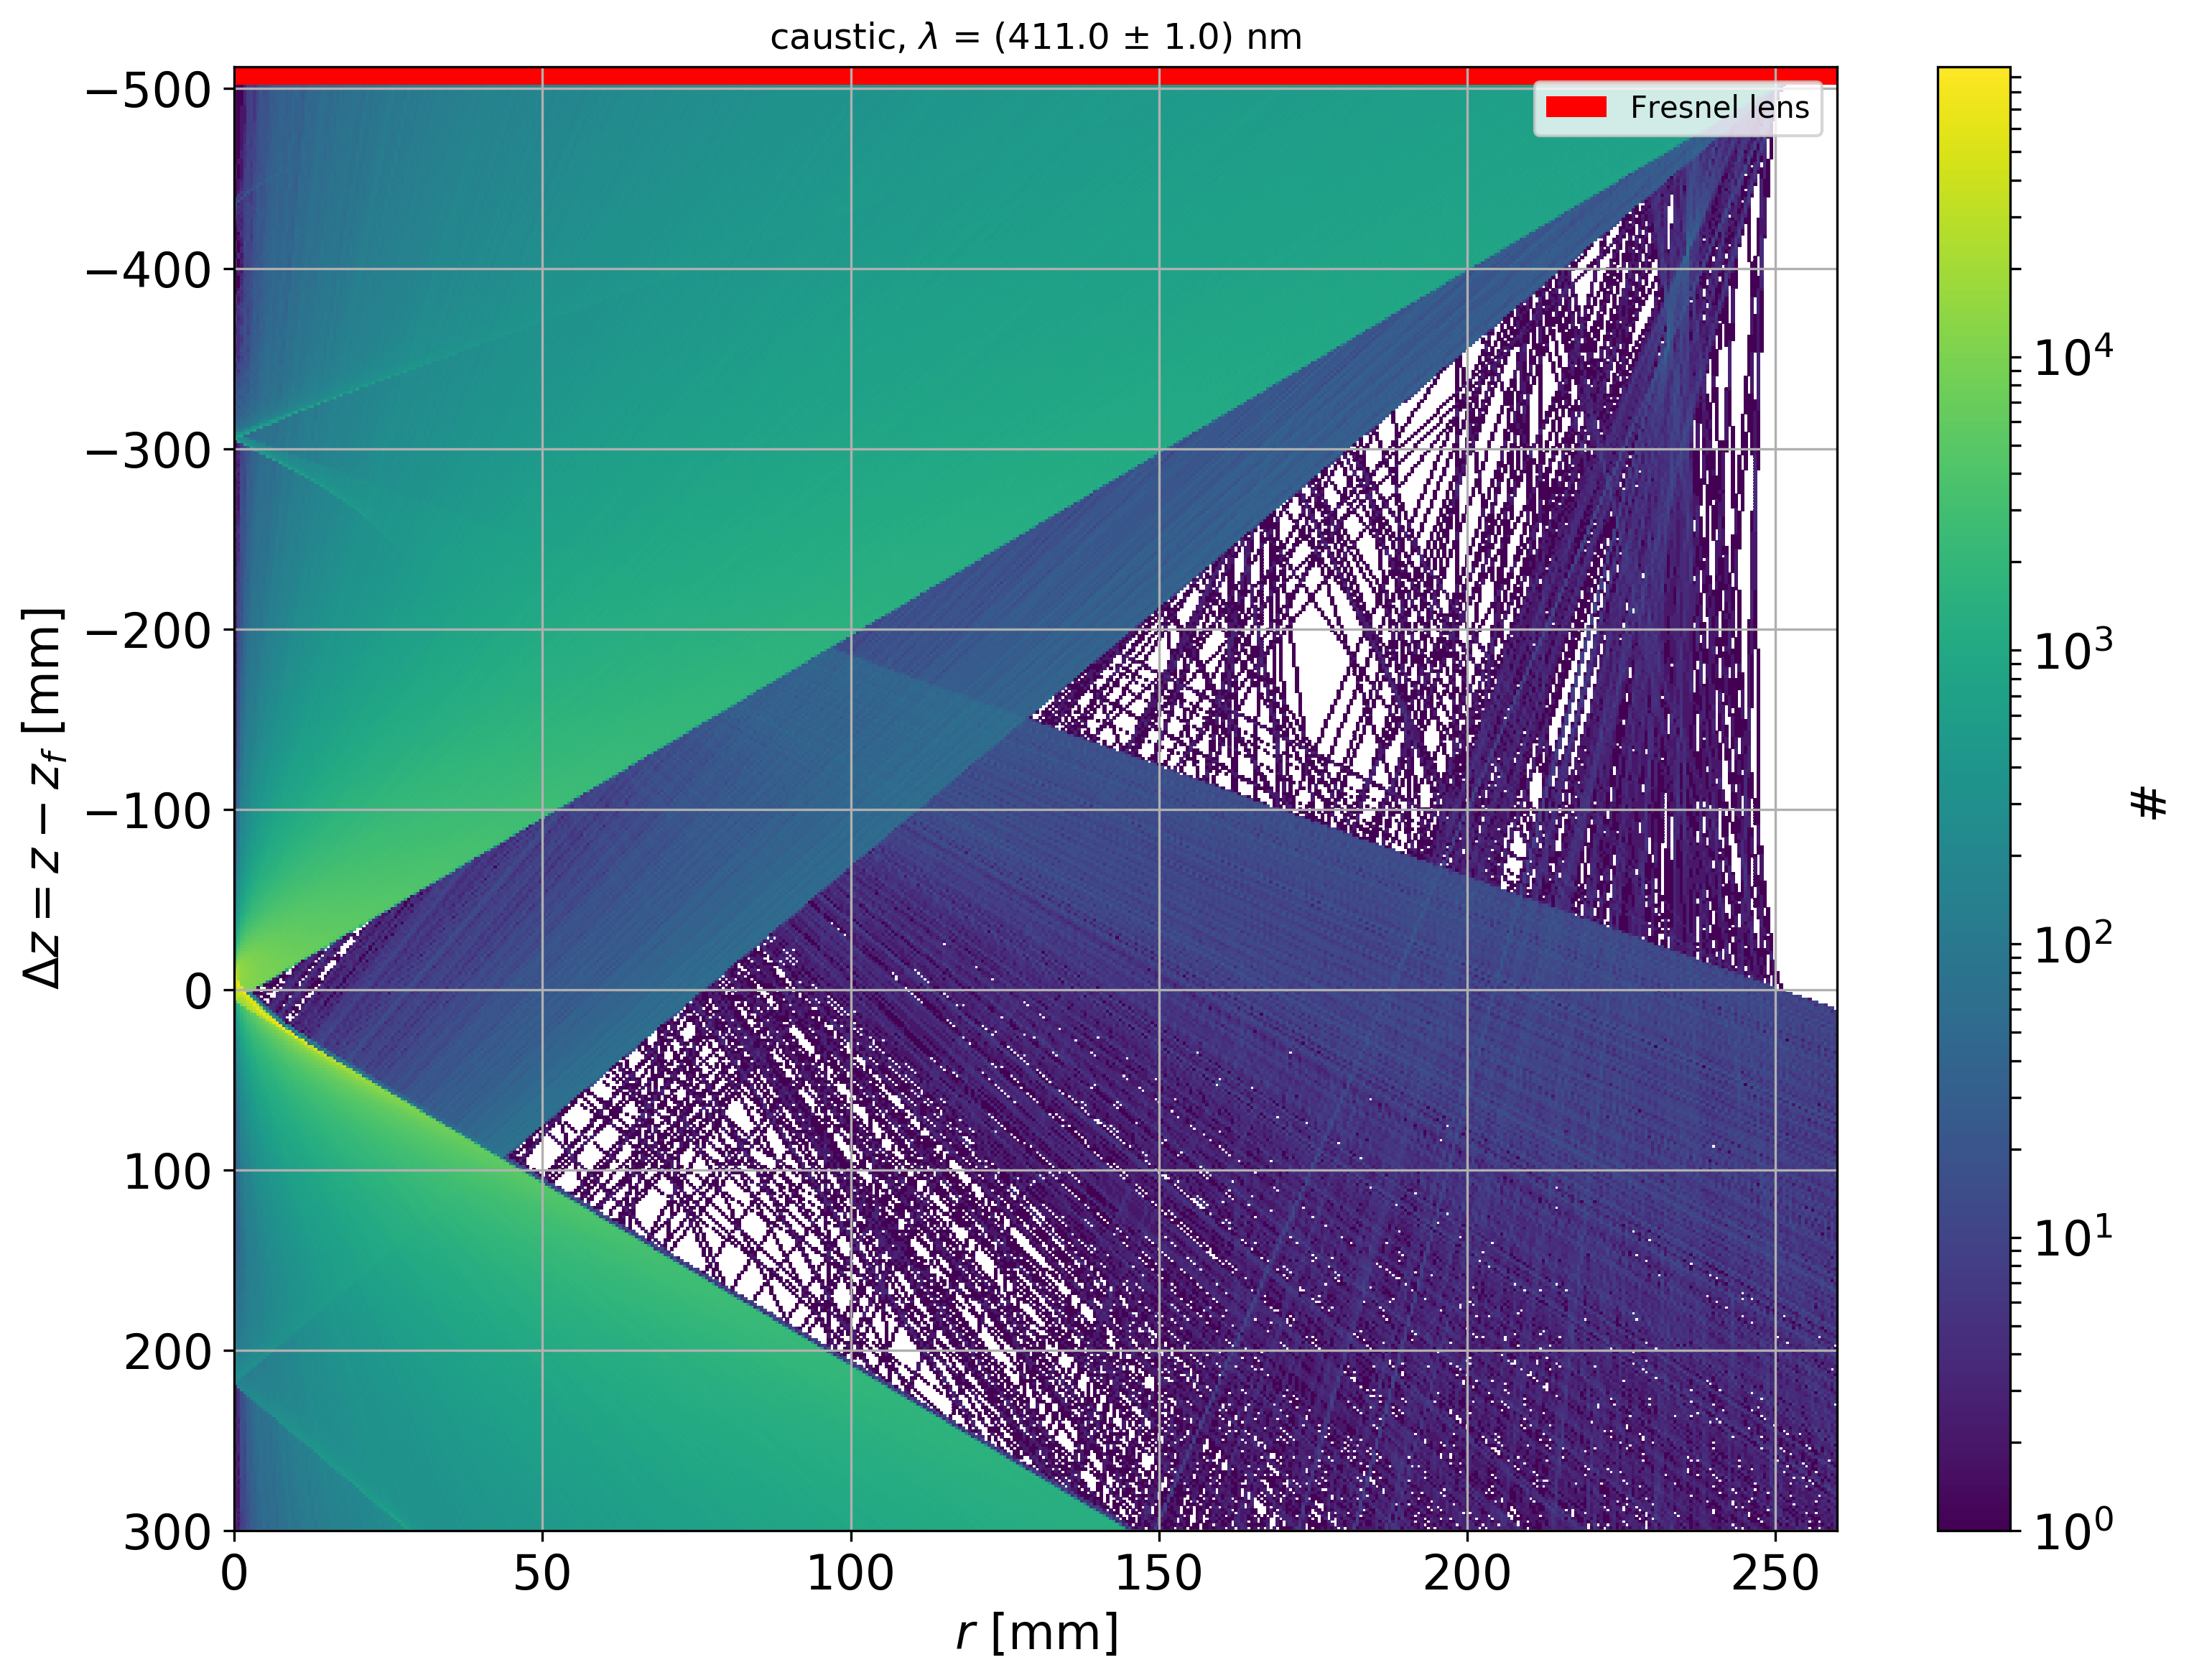
\includegraphics[width=0.8\textwidth]{focalplaneshift/caustic_411nm_zoomout.png}
	\caption[Zoomed-out caustic histogram]{\textbf{Zoomed-out caustic histogram.} The plot shows a zoomed-out version of figure~\ref{focalplaneshift_bestwvl}. The red band on the top denotes the location of the Fresnel lens. Besides a major focal spot at $\Delta z\approx\SI{0}{\milli\meter}$, one can see two minor ones at $\Delta z\approx\SI{-300}{\milli\meter}$ and $\Delta z\approx\SI{220}{\milli\meter}$ which come from the \enquote{false} refractions mentioned in section~\ref{iceact:model:fresnellens}.}
	\label{focalplaneshift_zoomout}
\end{figure}

\subsection{Winston Cone Simulation}



\section{Simulation Strategy and Verification}

\subsection{Winston Cone Meshing}\label{sec:wico_meshing}

\subsection{Aberration Effects -- \enquote{Ghost Image}}\label{sec:ghost_image}

\begin{figure}[H]
	\centering
	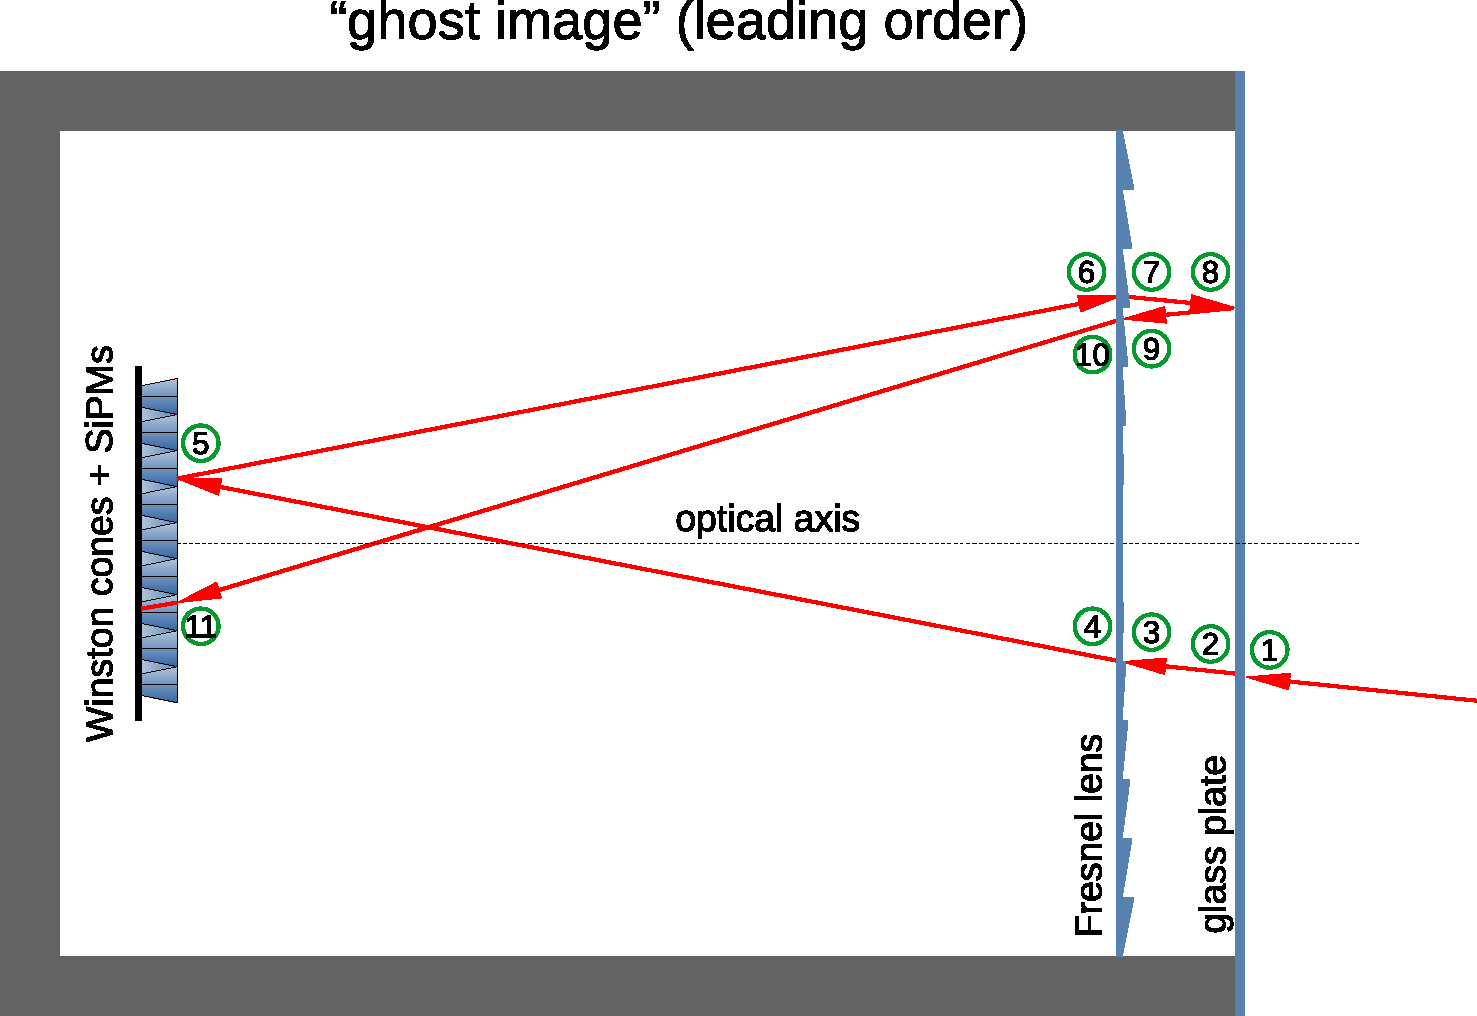
\includegraphics[width=0.9\textwidth]{GhostImage.pdf}
	\caption[Schematic sketch for the \enquote{ghost image} ray path]{\textbf{Schematic sketch for the \enquote{ghost image} ray path.} long caption}
	\label{ghostimage_path}
\end{figure}

\section{Parametrization Simulation}

\begin{figure}[H]
	\centering
	\saveimageheight[width=0.49\textwidth]{GeantCoords.pdf}
	\begin{subfigure}[t]{0.49\textwidth}
		\raiseimage[width=\textwidth]{CameraPixels.pdf}
		\subcaption{Top view of the \iceact camera with pixel numbering and coordinate system. The $z$-axis comes out of the drawing plane.}
	\end{subfigure}
	\hfill
	\begin{subfigure}[t]{0.49\textwidth}
		\usebox{\savedimage}
		\subcaption{Coordinate system for the \iceact telescope. The tube is sketched as a the blue cylinder. The coordinate origin is set as the center of the focal plane on the Winston cones' entrance windows. An exemplary incoming photon drawn as red line impinges on the glass plate under a zenith angle $\theta$ and an azimuth angle $\phi$.}
	\end{subfigure}
	\caption[Coordinate system used in \geant and for the simulation]{\textbf{Coordinate system used in \geant and for the simulation.} }
	\label{geant_coords}
\end{figure}